% ============================================================================
% SLIDE SEMINAR - BÁO CÁO TIẾN ĐỘ LUẬN VĂN THẠC SĨ
% Mạng Đối Nghịch Tạo Sinh Trong Chuyển Đổi Ảnh Chân Dung Sang Phong Cách Anime
% Nguyễn Trọng Nhân - 24025149
% Seminar: 22/07/2026
% ============================================================================

\documentclass[aspectratio=169,11pt]{beamer}

% === ENGINE DETECT & FONTS ===
\usepackage{iftex}
\ifXeTeX
  \usepackage{fontspec}
  \setsansfont{Arial}
  \usepackage[vietnamese]{babel}
\else
  \usepackage[utf8]{inputenc}
  \usepackage[utf8]{vietnam}
\fi

% === PACKAGES ===
\usepackage{graphicx}
\usepackage{booktabs}
\usepackage{amsmath,amssymb}
\usepackage{tikz}
\usepackage{xcolor}
\usepackage{hyperref}
\usepackage{multicol}
\usepackage{array}
\usepackage{colortbl}

% === THEME CONFIGURATION ===
\usetheme{Madrid}
\usecolortheme{whale}

% Custom UET colors
\definecolor{uetblue}{RGB}{0, 51, 102}
\definecolor{uetgold}{RGB}{204, 153, 0}
\definecolor{uetred}{RGB}{180, 0, 0}
\definecolor{lightblue}{RGB}{235, 243, 255}
\definecolor{resultgreen}{RGB}{0, 120, 50}

\setbeamercolor{structure}{fg=uetblue}
\setbeamercolor{palette primary}{bg=uetblue, fg=white}
\setbeamercolor{palette secondary}{bg=uetblue!85, fg=white}
\setbeamercolor{palette tertiary}{bg=uetblue!65, fg=white}
\setbeamercolor{frametitle}{bg=uetblue, fg=white}
\setbeamercolor{title}{fg=white, bg=uetblue}
\setbeamercolor{block title}{bg=uetblue, fg=white}
\setbeamercolor{block body}{bg=lightblue, fg=black}
\setbeamercolor{block title alerted}{bg=uetred, fg=white}
\setbeamercolor{block body alerted}{bg=uetred!10, fg=black}
\setbeamercolor{block title example}{bg=resultgreen!85, fg=white}
\setbeamercolor{block body example}{bg=resultgreen!10, fg=black}
\setbeamercolor{item}{fg=uetblue}
\setbeamercolor{footline}{bg=uetblue!90, fg=white}

% Font and Spacing settings
\setbeamerfont{title}{size=\Large, series=\bfseries}
\setbeamerfont{frametitle}{size=\large, series=\bfseries}
\setbeamerfont{footnote}{size=\tiny}

% Reduce spacing in lists and blocks
\setlength{\leftmargini}{1.2em}
\setlength{\leftmarginii}{1.0em}

% Remove navigation symbols
\setbeamertemplate{navigation symbols}{}

% Custom footline
\setbeamertemplate{footline}{
  \leavevmode%
  \hbox{%
  \begin{beamercolorbox}[wd=.35\paperwidth,ht=2.4ex,dp=1.1ex,center]{footline}%
    \usebeamerfont{author in head/foot}Nguyễn Trọng Nhân -- 24025149
  \end{beamercolorbox}%
  \begin{beamercolorbox}[wd=.42\paperwidth,ht=2.4ex,dp=1.1ex,center]{footline}%
    \usebeamerfont{title in head/foot}Báo cáo tiến độ Luận văn ThS
  \end{beamercolorbox}%
  \begin{beamercolorbox}[wd=.23\paperwidth,ht=2.4ex,dp=1.1ex,right]{footline}%
    \usebeamerfont{date in head/foot}\insertframenumber{} / \inserttotalframenumber\hspace*{2ex}
  \end{beamercolorbox}}%
}

% Graphics path
\graphicspath{{figures/}{figChap1/}{figChap2/}{figChap3/}{journal/figures/}{journal/phuluc/}}

% === METADATA ===
\title[GAN cho Anime hóa ảnh chân dung]{Mạng Đối Nghịch Tạo Sinh Trong Chuyển Đổi \\ Ảnh Chân Dung Sang Phong Cách Anime}
\subtitle{Seminar báo cáo tiến độ Luận văn Thạc sĩ}
\author[Nguyễn Trọng Nhân]{Học viên: \textbf{Nguyễn Trọng Nhân} -- 24025149 \\ GVHD: \textbf{TS. Ma Thị Châu}}
\institute[UET-VNU]{Trường Đại học Công nghệ -- ĐHQGHN}
\date{22/07/2026}

% ============================================================================
\begin{document}

% ============================================================================
% TITLE PAGE
% ============================================================================
{
\setbeamertemplate{footline}{}
\begin{frame}
\vspace{-0.2cm}
\begin{columns}
\begin{column}{0.12\textwidth}
\centering

\includegraphics[width=0.85\linewidth]{UET_logo.jpg}
\end{column}
\begin{column}{0.88\textwidth}
\centering
{\small ĐẠI HỌC QUỐC GIA HÀ NỘI}\\
{\small \textbf{TRƯỜNG ĐẠI HỌC CÔNG NGHỆ}}
\end{column}
\end{columns}
\vspace{0.1cm}
\titlepage
\end{frame}
}


% ============================================================================
% SLIDE 1: BÀI TOÁN & ĐỘNG LỰC NGHIÊN CỨU
% ============================================================================
\begin{frame}{1. Bài toán \& Động lực nghiên cứu}

\begin{columns}[T]
\begin{column}{0.56\textwidth}
\small
\textbf{Bài toán:} Chuyển đổi ảnh chân dung thực $\to$ anime, \textit{bảo toàn danh tính} và chạy \textit{thời gian thực} trên thiết bị cấu hình thấp.

\vspace{0.15cm}
\begin{block}{Thách thức hiện tại}
\begin{itemize}\itemsep=2pt
    \item \textbf{Mất chi tiết khuôn mặt (GANs):} CycleGAN, AnimeGANv2 xử lý toàn ảnh cùng độ phân giải $\Rightarrow$ ngũ quan bị mờ/méo khi mặt nhỏ trong ảnh.
    \item \textbf{Tốn chi phí tính toán (Diffusion):} Stable Diffusion + ControlNet đẹp nhưng nặng (2--7GB, 8--16GB VRAM, chỉ 0.5--2 FPS) $\Rightarrow$ khó triển khai mobile/web real-time.
\end{itemize}
\end{block}

\vspace{0.1cm}
\textbf{\textcolor{uetblue}{$\Rightarrow$ Mục tiêu đề tài:}} Xây dựng hệ thống \textbf{nhẹ (9.1MB), nhanh (42FPS), bảo toàn khuôn mặt}.

\end{column}
\begin{column}{0.41\textwidth}
\centering
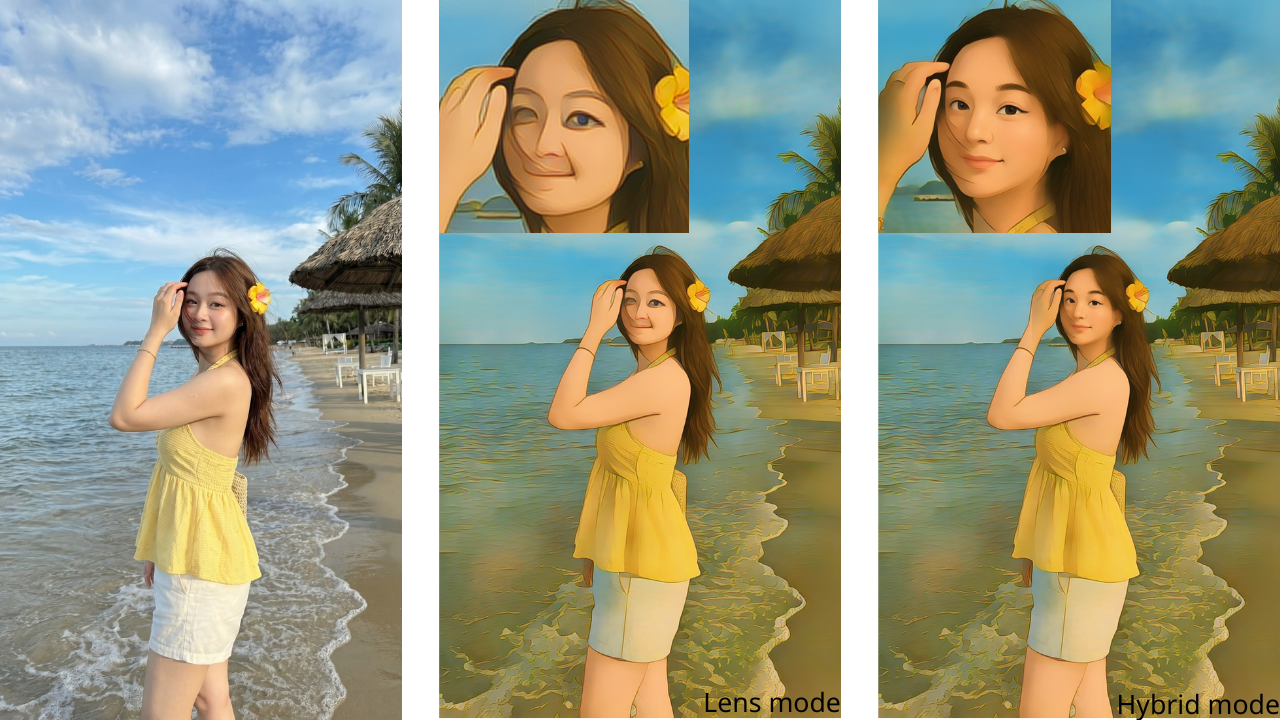
\includegraphics[width=0.95\linewidth]{anh3.png}

\vspace{0.05cm}
{\scriptsize Gốc $\to$ Landscape Mode $\to$ \textbf{Hybrid Mode}\\
(\textbf{Hybrid Mode} giữ nét ngũ quan tốt rõ rệt)}
\end{column}
\end{columns}

\end{frame}


% ============================================================================
% SLIDE 2: MÔ HÌNH ĐỀ XUẤT & ĐÓNG GÓP KỸ THUẬT
% ============================================================================
\begin{frame}{2. Mô hình đề xuất \& Thiết kế kỹ thuật}
\vspace*{-0.15cm}

\begin{columns}[T]
\begin{column}{0.54\textwidth}
\small

\begin{block}{Kiến trúc Face-Preserved Hybrid Framework}
\begin{itemize}\itemsep=1pt
    \item \textbf{Backbone:} DTGAN (AnimeGANv3) -- Double-Tail Generator với LADE normalization.
    \item \textbf{Face Detector:} RetinaFace MobileNet-0.25 ($\sim$500KB).
    \item \textbf{Adaptive Modes:} Face / Landscape / Hybrid mode.
\end{itemize}
\end{block}

\begin{block}{Thiết kế kỹ thuật chính}
\begin{itemize}\itemsep=1pt
    \item \textbf{Symmetric Margin Expansion:} Mở rộng bbox 50\%, ép 1:1, clamp biên ảnh $\to$ bảo toàn tóc, tai, cổ cho generator.
    \item \textbf{Feathered Blending:} Alpha compositing với mask Gaussian $\to$ ghép mặt HD vào nền mượt mà ($<$5ms/mặt).
\end{itemize}
\end{block}

\end{column}
\begin{column}{0.43\textwidth}
\centering
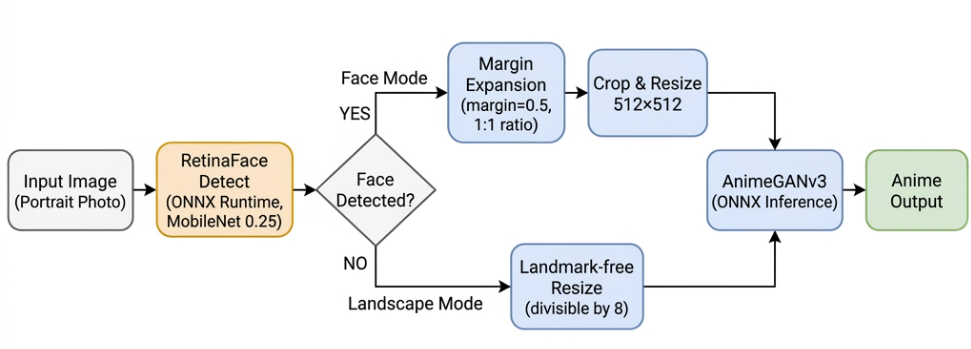
\includegraphics[height=1.6cm,keepaspectratio]{face_extraction_pipeline.png}

{\scriptsize Pipeline: RetinaFace $\to$ Margin $\to$ DTGAN $\to$ Blending}

\vspace{-0.1cm}
\begin{exampleblock}{\scriptsize Kết quả triển khai}
\scriptsize
\centering
\begin{tabular}{ll}
Kích thước & \textbf{9.1\,MB} (ONNX) \\
Tốc độ & \textbf{42\,FPS} \\
So với Diffusion & \textbf{200$\times$ nhỏ hơn}, \textbf{20$\times$ nhanh hơn}
\end{tabular}
\end{exampleblock}

\end{column}
\end{columns}

\end{frame}


% ============================================================================
% SLIDE 3: KẾT QUẢ THỰC NGHIỆM HIỆN TẠI
% ============================================================================
\begin{frame}{3. Kết quả thực nghiệm hiện tại}
\vspace*{-0.15cm}

\begin{columns}[T]
\begin{column}{0.48\textwidth}
\small

\begin{block}{So sánh định lượng (GAN baselines)}
\centering
\scriptsize
\begin{tabular}{lccc}
\toprule
\textbf{Phương pháp} & \textbf{FID}$\downarrow$ & \textbf{LPIPS}$\downarrow$ & \textbf{FPS} \\
\midrule
CycleGAN      & 98.4 & 0.512 & 18 \\
CartoonGAN    & 84.7 & 0.487 & 24 \\
AnimeGANv2    & 72.3 & 0.421 & 31 \\
\midrule
\textbf{Ours (Face)}  & \textbf{58.6} & \textbf{0.384} & \textbf{42} \\
\bottomrule
\end{tabular}
\end{block}

\vspace*{-0.1cm}
\begin{block}{Ablation Margin $m$}
\centering
\scriptsize
\begin{tabular}{cccp{2.2cm}}
\toprule
$m$ & FID$\downarrow$ & LPIPS$\downarrow$ & Nhận xét \\
\midrule
0.3 & 63.1 & 0.401 & Mất tóc/tai \\
\textbf{0.5} & \textbf{58.6} & \textbf{0.384} & Tối ưu ngữ cảnh \\
0.7 & 61.3 & 0.396 & Nhiễu nền \\
\bottomrule
\end{tabular}
\end{block}

\end{column}
\begin{column}{0.49\textwidth}
\small

\begin{block}{User Study (42 người tham gia)}
\begin{itemize}\itemsep=1pt
    \item \textbf{Phân nhóm:} 12 Experts + 30 Laypersons.
    \item \textbf{Ưa chuộng:} \textbf{88.8\%} ưu tiên Hybrid Mode.
    \item \textbf{Thống kê:} $p > 0.75$ (Mann-Whitney U).
\end{itemize}
\end{block}

\vspace*{-0.1cm}
\begin{exampleblock}{Đóng góp đạt được}
\begin{itemize}\itemsep=1pt
    \item Cải thiện \textbf{8.7\% FID} nhờ xử lý vùng mặt.
    \item Đạt tốc độ \textbf{42 FPS} trên GPU RTX A5000.
\end{itemize}
\end{exampleblock}

\end{column}
\end{columns}

\end{frame}


% ============================================================================
% SLIDE 4: KẾ HOẠCH HOÀN THÀNH LUẬN VĂN
% ============================================================================
\begin{frame}{4. Kế hoạch hoàn thành luận văn}

\begin{columns}[T]
\begin{column}{0.54\textwidth}
\small

\begin{block}{Các nhiệm vụ trọng tâm}
\begin{itemize}\itemsep=3pt
    \item \textbf{Hoàn thiện Luận văn:} Rà soát văn phong, kiểm tra định dạng Công văn 139/ĐT-2012 của UET.
    \item \textbf{Bài báo khoa học:} Hoàn thành bài báo tạp chí tiếng Anh (IEEE style), chuẩn bị nộp bài.
    \item \textbf{Chuẩn bị bảo vệ:} Đóng gói mô hình demo web/ONNX, hoàn thiện slide báo cáo chính thức.
\end{itemize}
\end{block}

\end{column}
\begin{column}{0.43\textwidth}
\small

\begin{block}{Timeline dự kiến}
\centering
\scriptsize
\begin{tabular}{p{2.3cm}p{2.8cm}}
\toprule
\textbf{Thời gian} & \textbf{Công việc} \\
\midrule
07/2026 & Rà soát LV + bài báo \\
08/2026 & Gửi GVHD phản biện \\
08--09/2026 & Chỉnh sửa hoàn thiện \\
09--10/2026 & Nộp hồ sơ \& Bảo vệ \\
\bottomrule
\end{tabular}
\end{block}

\begin{alertblock}{\small Lưu ý quản lý rủi ro}
\scriptsize
\begin{itemize}
    \item Dự phòng thời gian review bài báo.
    \item Đã chuẩn bị sẵn toàn bộ dữ liệu \& mã nguồn.
\end{itemize}
\end{alertblock}

\end{column}
\end{columns}

\end{frame}


% ============================================================================
% SLIDE 5: TIẾN ĐỘ VIẾT LUẬN VĂN ThS
% ============================================================================
\begin{frame}{5. Tiến độ viết Luận văn Thạc sĩ}

\begin{columns}[T]
\begin{column}{0.53\textwidth}
\small

\begin{block}{Tiến độ chi tiết từng phần}
\centering
\scriptsize
\def\arraystretch{1.05}
\begin{tabular}{lcc}
\toprule
\textbf{Nội dung} & \textbf{Trạng thái} & \textbf{Tiến độ} \\
\midrule
Mở đầu & Complete & 100\% \\
Ch.1: Cơ sở lý thuyết & Complete & 100\% \\
Ch.2: Kiến trúc DTGAN & Complete & 100\% \\
Ch.3: Face Extraction Pipeline & Complete & 100\% \\
Ch.4: Thực nghiệm \& Đánh giá & Complete & 100\% \\
Ch.5: Kết luận & Complete & 100\% \\
Bìa, Phụ bìa, Phụ lục & Complete & 100\% \\
\midrule
\textbf{Bài báo Journal (IEEE)} & \textbf{Drafting} & \textbf{85\%} \\
\bottomrule
\end{tabular}
\end{block}

\end{column}
\begin{column}{0.44\textwidth}
\small

\begin{exampleblock}{Tổng kết Luận văn}
\begin{itemize}\itemsep=2pt
    \item \textbf{Bản thảo Luận văn:} Đã viết xong 6/6 chương.
    \item \textbf{Định dạng:} Đúng chuẩn UET (Công văn 139/ĐT).
\end{itemize}
\end{exampleblock}

\begin{block}{Tiến độ Bài báo Journal}
\begin{itemize}\itemsep=2pt
    \item \textbf{Tạp chí:} IEEE (dự kiến).
    \item \textbf{Tiêu đề:} \textit{Face-Preserved Hybrid Framework...}
    \item \textbf{Đã viết:} Abstract, Intro, Method, Exp, Conclusion (85\%).
\end{itemize}
\end{block}

\end{column}
\end{columns}

\end{frame}


% ============================================================================
\begin{frame}{}
\centering
\vfill
{\LARGE \textbf{Cảm ơn Thầy/Cô và các anh/chị!}}

\vspace{0.5cm}
{\large Nguyễn Trọng Nhân -- 24025149}\\
{\normalsize GVHD: TS. Ma Thị Châu}\\
\vspace{0.3cm}
{\small Email: 24025149@vnu.edu.vn}
\vfill
\end{frame}

\end{document}
